%%%%%%%%%%%%%%%%%%%%%%%%%
% Set up to be stand alone document
% All declerations in the header to be removed when added into thesis
%%%%%%%%%%%%%%%%%%%%%%%%%
\documentclass[12pt]{article}

\usepackage{booktabs} % booktabs provides professional formatting commands for tables
\usepackage{amsmath} % amsmath provides extra maths symbols
\usepackage{textcomp} % textcomp provides extra text symbols (like a degrees celsius symbol)
\usepackage{../customisations}
\usepackage{natbib}

\title{$J$-band Sythentic Spectral Fitting}
\date{\today}

\begin{document}
\maketitle
%%%%%%%%%%%%%%%%%%%%%%%%%
% To be included when added into thesis
% \chapter{J-band Sythentic Spectral Fitting}

In this chapter I describe in detail the process by which I implement an analysis
routine to fit RSG sythetic spectra to observed data.
The spectra cover the $J$-band, spectifically the $1.16-1.22\mu$m region, where there are various prominent spectral features.
These spectral features, arising from elemental absorption, are compared in the observed and model spectra,
where the $\chi^{2}$-statistic is calcualted to asses the goodness of fit for each model.
The stellar parameters which are fit for in this analysis are global metallicitiy [Z], effective temperature (T$_{eff}$), microturblance ($\xi$) and surfance gravity ($log g$).
% In addition to these parameters, in the future I also hope to further develop this implementation to include the $\alpha$-to-iron ratio as a free parameter.
The observed spectra are fit with model spectra from a set of MARCS model atmospheres
\cite{2008A&A...486..951G}.

The wavelength range, over which to perform this analysis,
is chosen based on the spectral appearance of the region.
Typically, in the spectra of cool stars, dense molecular absorption fetuares dominate the spectrum which require high-resolution spectroscopy to distinguish individual features and derive stellar parameters~\cite{Cunha07, Davies09a, Davies09b}.
However, in this small wavelength range, the absorption is dominated by well separaeted elemental absorption features from iron, magnesium, silicon and titanium.
Therefore, the spectral resolution required in order to derive stellar paramters is significantly reduced.
This means that this analyis can be preformed with a relatively small amount of telescope time using multi-object spectrographs like the $K$-band multi-object spectrograph (KMOS)
or the multi-object spectrometer for infra-red exploration (MOSFIRE) and is therefore feasible for studies of red supergiant stars (RSGs) in external galaxies.

In addition to this, given the cool temperature of the outer layers of RSGs,
the peak brightness of a typical RSG is $\sim1.1\mu$m.
Combining this with the fact that dust attenuation is significanlty lower in the near-IR, compared to the optical regime, RSGs are ideal candidates to be studied at large distances.

Previous implemenations of this analysis include that of
\cite{2010MNRAS.407.1203D} and Gazak (2014).
This implemenation includes aspects of both of these previous implementations and could be described as a hybrid of the two.
I approach the implementation in a Bayesian manor which relies on good prior assumptions.
Eventually this analysis routine will be made publicly available which should encourage the community to engage with these routines.

In the remainder of this chapter I first describe the model grids and how they are used in~\ref{sub:model_grid}.
I then describe the contiuum fitting procedure in~\ref{sub:continuum_fitting},
and go on to detail the method for estimating the bestfit parameters in
~\ref{sub:best_fit_parameters}.
The testing process which these procedures have underwent is described in~\ref{sub:testing}, which also includes a comparison between the results produced using this implementation and those of the two previous implementations of the same analysis.
Finally, I conclude the chapter in~\ref{sub:conclusions}.

% Based on the work done by \cite{2010MNRAS.407.1203D} and Gazak (2014), I developed an implementation of the J-band synthetic spectral fitting software.
% This involves fitting the continuum between the observations and models and defining best fit model parameters for the stellar parameters,
% metallicity, effective temperature, surface gravity and microturbulence.
% The observations are fit with model spectra from a set of MARCS model atmospheres
% \cite{2008A&A...486..951G}.
% Spectra are extracted using the SUI code
% ~\cite{2012ApJ...751..156B,2013ApJ...764..115B,2014arXiv1412.6527B}
% with non-LTE corrections computed for iron, silicon and titanium.

\subsection{Model Grid} % (fold)


\label{sub:model_grid}
\begin{itemize}
    \item How are the grids generated?
    \item What are the non-LTE corrections?
Spectra are extracted using the SUI code
~\cite{2012ApJ...751..156B,2013ApJ...764..115B,2014arXiv1412.6527B}
with non-LTE corrections computed for iron, silicon and titanium.
    \item What do the current grids look like?
    \item How could they be improved?
\end{itemize}
% subsection model_grid (end)
\subsection{Continuum Fitting} % (fold)
\label{sub:continuum_fitting}

Accurately matching the continuum levels in the models with that of the observed
spectrum provides a base with which to anchor the diagnostic lines.
An incorrecly placed continuum level would bias the analysis and result in the
strength of the diagnostic lines being over or under estimated producing inaccurate stellar parameters.

% The continuum fitting procedure is important because determining the base of the
% diagnostic lines defines their overall strength which is used to distinguish
% between models.
There are many factors that affect the level of the continuum and continuum placement,
including the resolution of the observations as well as the stellar parameters themselves.
Therefore it is vital that when attempting to derive stellar paramters,
in crowded regions such as this, the continuum placement is performed
consistently and accurately.
Intrinsically, when stufying RSGs at medium resolution - owing  to their cool atmospheres -
there are may instances of blended spectral features.
At this resolution the density of spectral features creates a pseudo-continuum which in practice is never at the ture continnum level.
Figure~\ref{fig:mod-res} illustrates the varying continuum levels for models where the resolution is varied and
Figure~\ref{fig:mod-z} shows this affect when varying only the metallicity.

\begin{figure}
 \centering
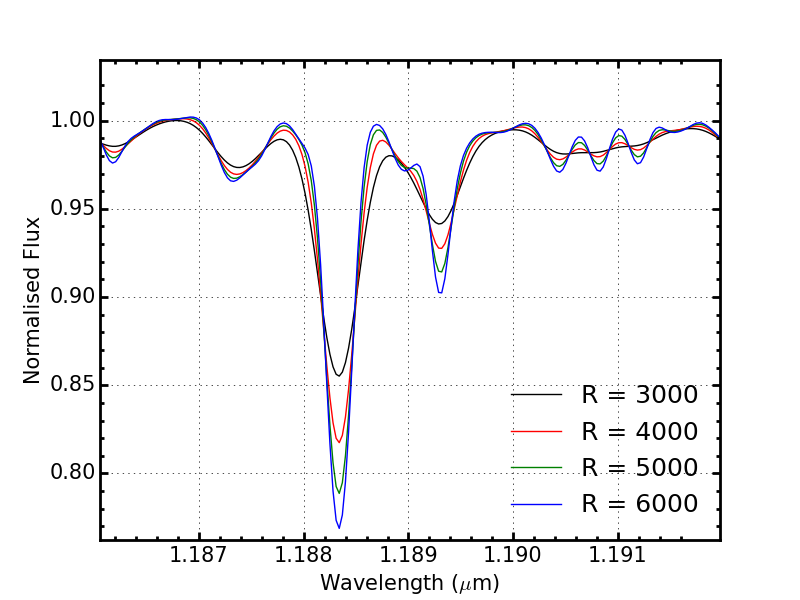
\includegraphics[width=\textwidth]{Resolution}
\caption{
One model degraded to four different resolution values.
This figure demonstrates the how the continuum level changes depending upon
the resolution of the spectrum.
We see at around 1.191$\mu$m at $R=3000$ the continuum level is perturbed by blended lines.
\label{fig:mod-res}
         }
\end{figure}

\begin{figure}
 \centering
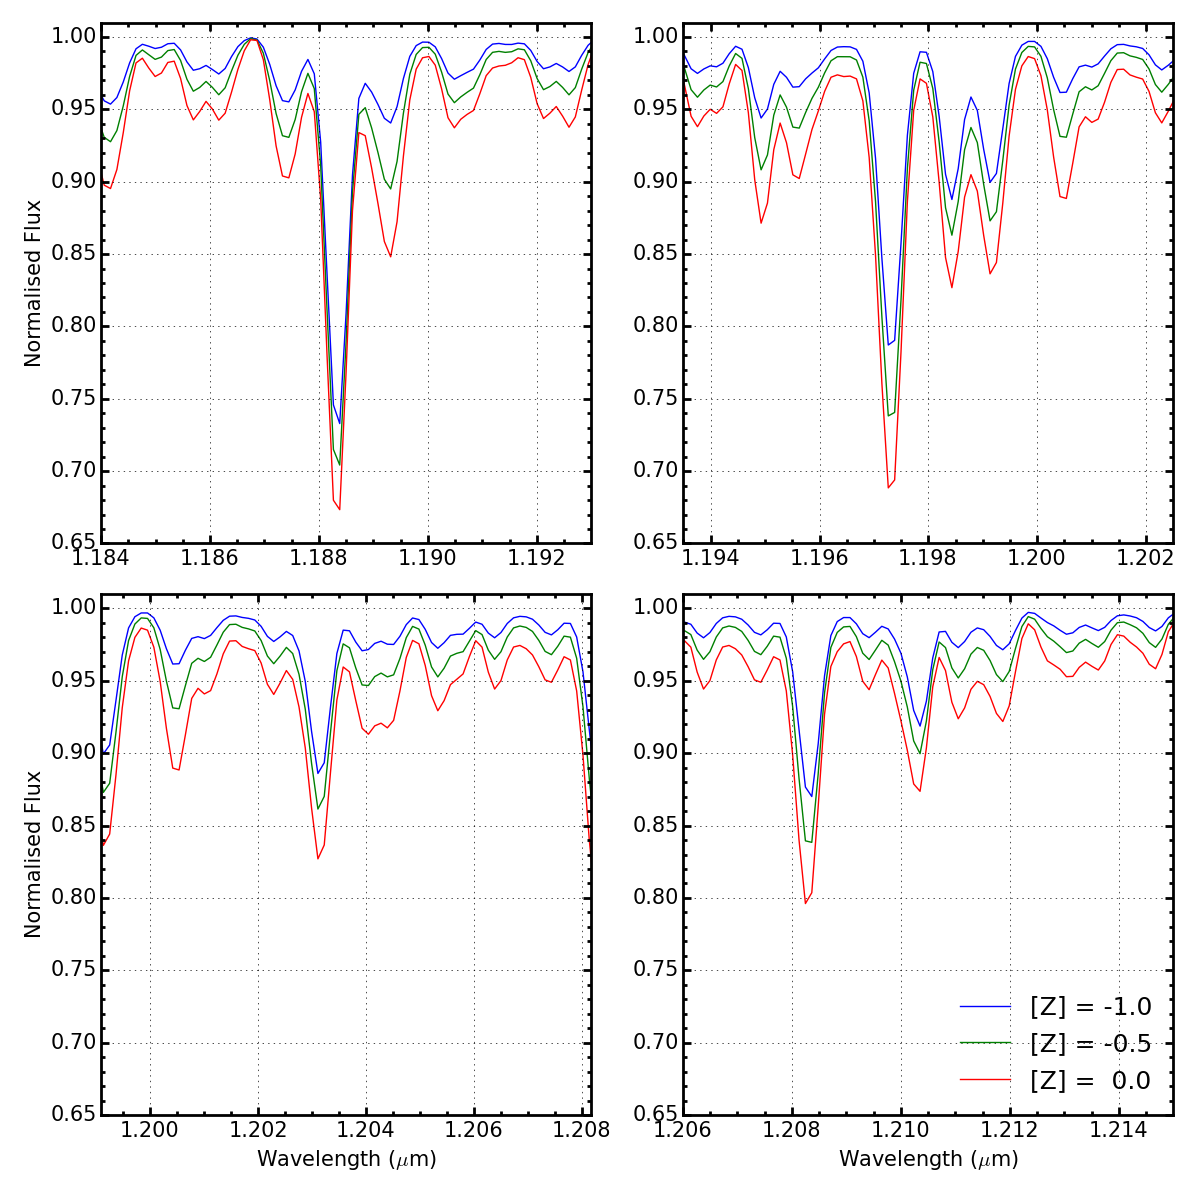
\includegraphics[width=\textwidth]{varyZ}
\caption{
Three models where only the metallicitiy is varied.
Each panel shows one or more diagnostic line.
Metallicity of the model intrinsically affects the continuum level of the spectrum,
such that at higher metallicities, there is greater departure from the true continuum level, which in the case of the models is 1.00.\label{fig:mod-z}
         }
\end{figure}


Given that it is impossible to know the true continuum level from any given observation,
the scaling applied must be consistent between the models and observations.
Scaling is required not only to match the levels of the continnum placement, but also to match the line strenghts between the models and observations.
Providing the treatment of the models and observations are consistent, the fact that the true continuum is never attained is not significant
\citep{2014ApJ...788...58G}.
For this procedure to work effectively, the observed and model spectra should be at the same resolution, have a consistent wavelength calibration and spectral sampling.

In order to account for difference between the spectral sampling in the observed and model spectra,
each model spectrum is resampled onto the wavelength scale of the observations by means of a linear interpolation routine.
The model spectrum is then degraded to the resolution of the observations by convolving this spectum with a gaussian filter where the width of the gaussian Is defined by the observed resolution.
The resolution of the KMOS observations is estimated using the KMOS/esorex pipeline from arc lamp exposures at the appropriate rotator angle for the observations.
This is measured for each spectrograph and is assumed to be constant (to within $\pm 100$) across individual IFU's as well as across the detector.

% This is accounted for by degrading the sampling of the models to that of the observations by means of a linear interpolation.
% The sampling of the models are degraded to that of the observations by means of a cublic-spline interpolation.
To ensure the spectra are on the same wavelength scale, the observed specturm is cross-correlated with the model spectrum;
a shift is then applied to the observed spectrum in order to minimise the cross-correlation matrix.
Over this small wavelength range, one would not expect significant variations in the spectral resolution of the observations to pertrub the cross-correlation.


To fit the continuum of the observations first I define the continuum width ($cw$) as:

\begin{equation}
    cw = \frac{\lambda}{R}, %\times S,
\end{equation}
\noindent where $R$ is the resolution of the spectrum and
$\lambda$ is the wavelength at which the width is taken
(in principle this wavelength varies across the spectrum, however, given our spectral window is sufficently small, I assume $\lambda = 1.20\mu$m).
% and $S$ is a scale factor which takes the range $0.5 < S < 1.0$.
The continuum width is essentially the resolution element of the spectrum at a wavelength of $\lambda = 1.20\mu$m.
 % multiplied by the scale factor $S$.
% In Gazak et al. (2015) this scale factor is fixed at 0.5.
% The scale factor is introduced because ... ?

The model spectrum is divided into wavelength slices each of width $cw\mu$m and the maximum of each slice is taken.
Figure~\ref{fig:cw} illustrates that using this technique systematically removes absorption features from the spectrum.
In this figure blue points represent the boundaries between the slices of witdh $cw\mu$m and the maximum of each slice is shown in red.
Any remaining features in this maximum spectrum are removed by rejecting outliers which are more than 3$\sigma$ from the mean of the distribution.
In figure~\ref{fig:cw} the $cw~max.$ points have been through this procedure.
This can be seen by noting that the cores of the absorption lines no $cw max.$
points present.

\begin{figure}
 \centering
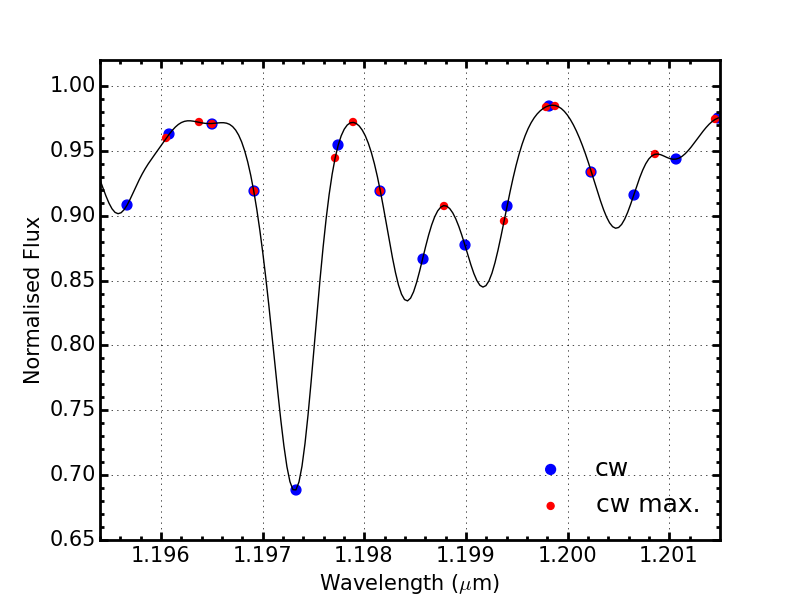
\includegraphics[width=\textwidth]{cw}
\caption{
Illustration of the continuum width ($cw$) and slicing the model spectrum into regions of $cw\mu$m is able to remove structure in order to fit the continnum.
The solid black line shows an example of a model spectrum degraded to a resolution of 3000,
blue points show the boundaries between the slices and red points show the maximum of each slice.\label{fig:cw}
         }
\end{figure}



The remaining data points ($P_{cont}$) are used to derive an inital correction function
($cf_{1}$) defined using the equation:
\begin{equation}
    cf_{1} = f(\frac{F_{mod}(P_{cont})}{F_{obs}(P_{cont})})
\end{equation}

\noindent where $F_{mod}$ and $F_{obs}$ are the flux in the model and observed spectrum respectively.
The final correction function ($cf_{2}$), a refinement of $cf_{1}$,
is defined by removing outliers more than 3$\sigma$ from the mean of the correction function $cf_{1}$.
This function is used to define the amount of scaling required for the model.


% The green dashed line shows a third order polynomial fit to the ratio of the model spectrum to a simulated observed spectrum at only the red points ($ = \frac{F_{mod}(cf_{1})}{F_{obs}(cf_{1})}$).

Alternative methods of continuum fitting are discussed in~\cite{2010MNRAS.407.1203D} and~\cite{2011A&A...527A..50E}.
These methods select pseduo-continuum pixels in the models based on ranking the model pixels and selecting a percentage of the pixels with the largest flux.
Providing the pixels from the model are selected in this manor and not those in the observations, this is a reliable method with which to derive the continuum level as demonstrated by Davies et al. (2015 in prep.).
\textbf{What advantage (if any) does the method applied here have over the one used in Davies et al. (2015 in prep.)?}

% subsection continuum_fitting (end)
\subsection{Best Fit Parameters} % (fold)
\label{sub:best_fit_parameters}

Bestfit paramaters are calcaulted using a chi-squared minimisation approach.
Each model in a $21\times19\times11\times9$ model grid is compared to the observed spectrum
and a chi-squared value is calculated using the equation,

\begin{equation}
    \chi^{2} = \frac{1}{N_{pix}}\sum{\frac{(O_{i} - M_{i})^{2}}{\sigma^{2}}}
\end{equation}

where $N_{pix}$ is the number of pixels used and
$\sigma$ is determined by the S/N of the spectrum.
Table~\ref{tb:lines} details the diagnostic lines used in this analysis.
The wavelength range over which to compute the $\chi^{2}$ is important to consider.
If the range is too small, the wings of the lines will be neglected,
which would lose vital information which is used to contstrain the model parameters.
For example, microturblance most affects the wings of the diagnostic lines.
\textbf{Confirm this!}
However, if too much of the psuedo-continuum is included, the parameters could be biased by noise features in the observations.
The regions which are taken  for the $\chi^{2}$ calculation is shown in figure~\ref{fig:lines}.
There are multiple cases where the diagnostic lines are sufficiently close together that, at R$\sim$3000

\begin{figure}
 \centering
 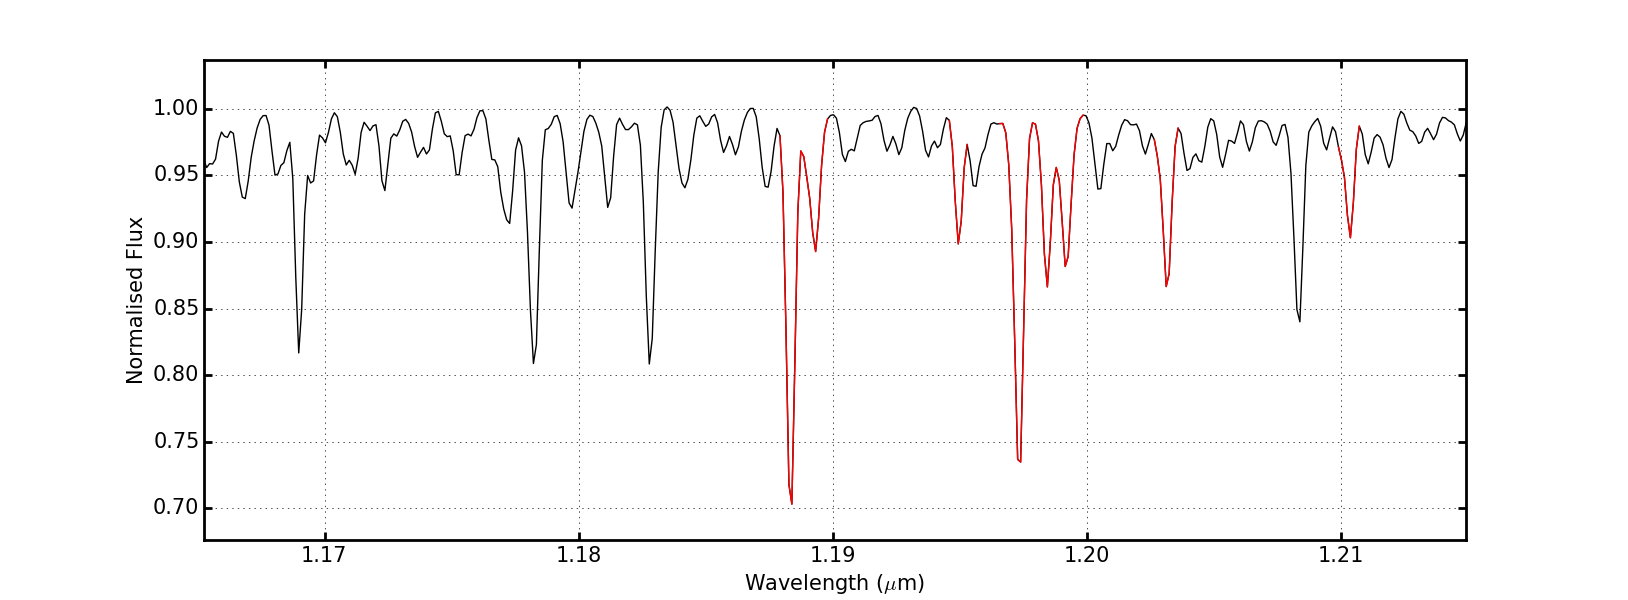
\includegraphics[width=\textwidth]{Diag-lines}
 \caption{
An example of a model spectrum, degraded and resampled to that of a typical observed spectrum (in this case NGC6822-RSG01), where the regions used to compute the $\chi^{2}$ calculation is highlighted in red.\label{fig:lines}
         }
\end{figure}


Each observed spectrum is cross-correlated before the $\chi^{2}$ calculation is performed with a rest wavelngth spectrum.
Additionally, each observed-model spectra pair is cross-correlated prior to the calculation, an estiamte of the offset between the two spectra is calcualted using an iterative approach and the offset is applied to the observed spectrum to ensure the central wavelengths of the lines are at rest wavelenght.
The cross-correlation shift between each observed-model spectra pair is typically $\sim$0.01pix.

Each parameter is selected based on a weighted average, where the weights are
determined by the $\chi^{2}$ value of the model:

\begin{equation}
    w = exp(-\chi^{2}/2)
\end{equation}

\begin{table}
\caption{Diagnostic lines\label{tb:lines}}
\scriptsize
\begin{center}
\begin{tabular}{cc}
 \hline
 \hline
Species & Line Centre \\
 \hline
Fe\,I & 1.188285 \\
Fe\,I & 1.197305 \\
Si\,I & 1.198419 \\
Si\,I & 1.199157 \\
Si\,I & 1.203151 \\
Si\,I & 1.210353 \\
Ti\,I & 1.189289 \\
Ti\,I & 1.194954 \\
Mg\,I & \\
Mg\,I & \\
 \hline
\end{tabular}
\end{center}
\end{table}

The average is performed over 100 models with the lowest $\chi^{2}$ value.
\textbf{Need to define some parameter stability tests and show that 100 is a
good amount of models to use.}

Errors on the parameters are determined by defining
$\Delta\chi^{2} = \chi^{2}_{min} + 3$.
The standard deviation of the models parameters for all models which have a
$\chi^{2}$ value within this range define the errors.

The significance of the 3 is that given that there are 8 diagnostic lines,

\subsection{Testing} % (fold)
\label{sub:testing}

% subsection testing (end)

\subsection{Conclusions} % (fold)
\label{sub:conclusions}

% subsection conclusions (end)
% subsection best_fit_parameters (end)
\bibliography{journals}{}
\bibliographystyle{apalike}
%%%%%%%%%%%%%%%%%%%%%%%%%
% To be removed when added into thesis
\end{document}
%%%%%%%%%%%%%%%%%%%%%%%%%